\documentclass[border=3mm]{standalone}
    \usepackage{tikz}
    \usetikzlibrary{backgrounds,shadows,positioning,fit,matrix,shapes.geometric, shapes.arrows} % add shadows #1

    % a way to cut shadows in a cell #2
    %https://tex.stackexchange.com/questions/129318/remove-drop-shadow-from-one-node
    \makeatletter
    \tikzset{no shadows/.code=\let\tikz@preactions\pgfutil@empty}
    \makeatother

    \tikzset{background/.style={rectangle, fill=red!10, inner sep=0.2cm},
              backgroundN/.style={rectangle, fill=white, inner sep=0.3cm},
              backgroundNN/.style={rectangle, fill=red!10, inner sep=0.2cm}}
	
	\tikzset{back/.style={rectangle, fill=blue!10, inner sep=0.2cm},
	              backgroundN/.style={rectangle, fill=white, inner sep=0.3cm},
	              backgroundNN/.style={rectangle, fill=red!10, inner sep=0.2cm}}
	              	
    \definecolor{mybluei}{RGB}{124,156,205}
    \definecolor{myblueii}{RGB}{73,121,193}
    \definecolor{mygreen}{RGB}{202,217,126}
    \definecolor{mypink}{RGB}{233,198,235}
\definecolor{antiquefuchsia}{rgb}{0.57, 0.36, 0.51}
\definecolor{byzantium}{rgb}{0.44, 0.16, 0.39}
\definecolor{darkcandyapplered}{rgb}{0.64, 0.0, 0.0}
\definecolor{darkbyzantium}{rgb}{0.36, 0.22, 0.33}
\definecolor{jasper}{rgb}{0.84, 0.23, 0.24}
\definecolor{pastelred}{rgb}{1.0, 0.41, 0.38}
\definecolor{pinkpearl}{rgb}{0.91, 0.67, 0.81}
\definecolor{blue(pigment)}{rgb}{0.2, 0.2, 0.6}

    \newcommand\widernode[5][widebox]{
    \node[
        #1,
        fit={(#2) (#3)},
        label=center:{\sffamily\bfseries\color{black}#4}] (#5) {};
    }

    \begin{document}

    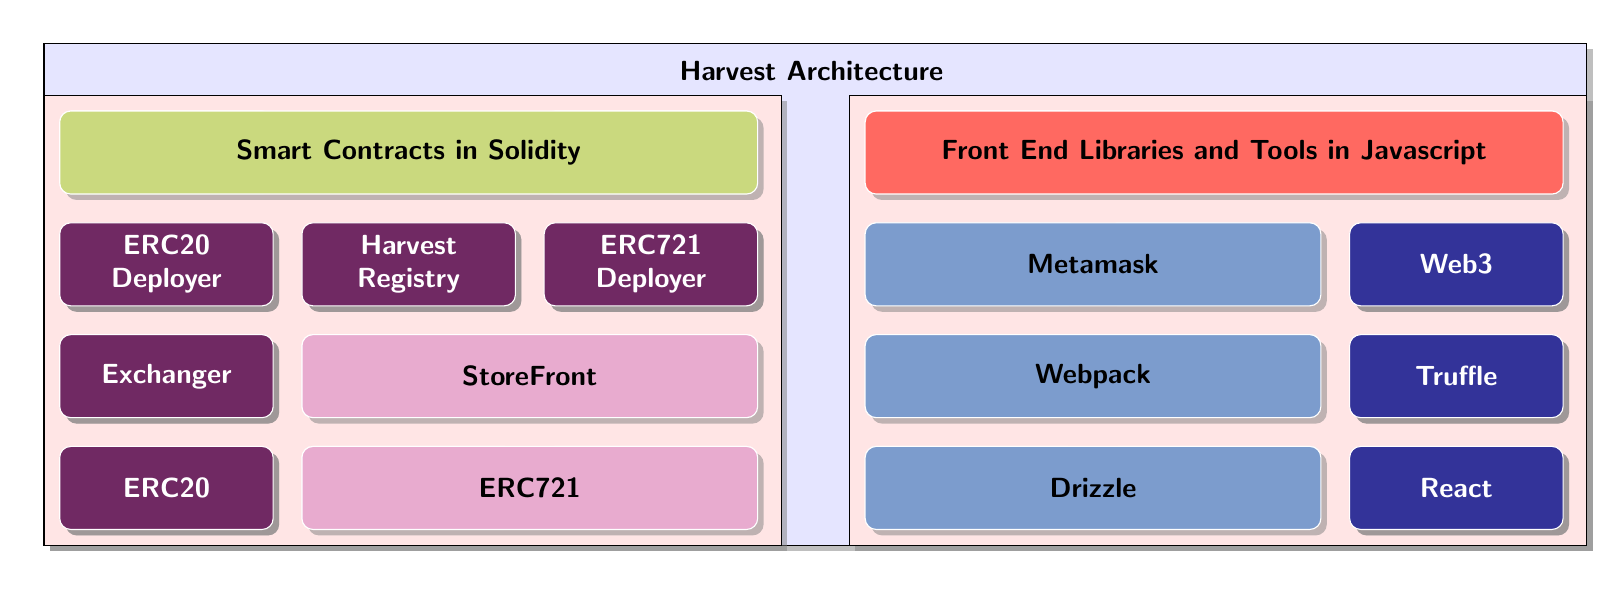
\begin{tikzpicture}[node distance=2pt,outer sep=0pt, % just do nothing after modification
    boxstyle/.style={
    draw=white,
    fill=#1,
    rounded corners, drop shadow, %to get a shadow in below a node
    font={\sffamily\bfseries\color{white}},
    align=center,
    minimum height=30pt
    },
    box/.style={
    boxstyle=#1,
    text width=2.5cm},
    box/.default=mybluei,
    title/.style={font={\sffamily\bfseries\color{black}}},
    widebox/.style={draw=white,inner sep=0pt, rounded corners,fill=#1,drop shadow},
    widebox/.default=mybluei,
    mylabel/.style={font={\sffamily\bfseries\color{black}}},
    database/.style={
      cylinder,
      cylinder uses custom fill,
      cylinder body fill=yellow!50,
      cylinder end fill=yellow!50,
      shape border rotate=90,
      aspect=0.25,
      draw
    }
    ]


    \matrix (stack) [%  boxstyle=mybluei!40,%will overpaint blocks with background
    column sep=10pt, row sep=10pt, inner sep=4mm,%
        matrix of nodes,
            nodes={box, outer sep=0pt, anchor=center, inner sep=3pt},%  
            nodes in empty cells=false,% #3
        row 1/.style={nodes={fill=none,draw=none,minimum height=3mm}},
    ]
    {
    |[no shadows]| & & & [1cm] & & |[no shadows]| \\ % #5
    %RCP main & Authoring & Browsing & Publishing & Search&|[no shadows]| \\
    |[no shadows]| & & |[no shadows]| & |[no shadows]|&  &|[no shadows]| \\
    |[box=byzantium]| ERC20 Deployer & |[box=byzantium]| Harvest Registry & |[box=byzantium]| ERC721 Deployer &|[no shadows]| & |[no shadows]|& |[box=blue(pigment)]| Web3 \\
     |[box=byzantium]| Exchanger & |[no shadows]| &|[no shadows]| & |[no shadows]| &|[no shadows]| & |[box=blue(pigment)]| Truffle \\
    |[box=byzantium]| ERC20 & |[no shadows]| & |[no shadows]| & |[no shadows]| & |[no shadows]| & |[box=blue(pigment)]| React \\};


    \widernode[]{stack-1-1}{stack-1-6}{Harvest Architecture}{EPF} %#5
	
	\widernode[widebox=mygreen]{stack-2-1}{stack-2-3}{Smart Contracts in Solidity}{SM}
	
	\widernode[widebox=pastelred]{stack-2-4}{stack-2-6}{Front End Libraries and Tools in Javascript}{FE}
	
    \widernode{stack-3-4}{stack-3-5}{Metamask}{MM}
  % \widernode{stack-3-6}{stack-3-6}{Web3}{AA}
    \widernode{stack-4-4}{stack-4-5}{Webpack}{BB}
  %  \widernode{stack-4-6}{stack-4-6}{Truffle}{CC}
    
    \widernode{stack-5-4}{stack-5-5}{Drizzle}{DC}
  %  \widernode{stack-5-6}{stack-5-6}{React}{MC23}
    
    %\widernode[widebox=pinkpearl]{stack-4-1}{stack-4-1}{Exchanger}{UMA23}
    \widernode[widebox=pinkpearl]{stack-4-2}{stack-4-3}{StoreFront}{UMA}
    %\widernode{stack-4-4}{stack-4-5}{Export/Import}{ExImp}
    \widernode[widebox=pinkpearl]{stack-5-2}{stack-5-3}{ERC721}{EMF}
    %\widernode[widebox=mygreen]{stack-6-1}{stack-6-5}{RCP Runtime}{RCPrun}


%    \widernode[widebox, text width=1.5cm, align=center]{stack-2-6}{stack-3-6}{Normal text works}{NTWorks}
%

    %\node [fit={(stack.south west)(stack.south east)},boxstyle=myblueii,draw=black,inner sep=0pt,below=3pt of stack.south,anchor=north,label={[mylabel]center:Java Runtime}] (JavaR) {};

%
%

%
		
		\begin{pgfonlayer}{background}
		        \coordinate (aux) at ([xshift=1mm]stack-5-6.east);
		            \node [back,
		                fit=(stack-1-1) (stack-5-1) (aux), draw, drop shadow,
		            ] {};
		            %\node [backgroundN,
		            %    fit=(stack-3-5) ] {};
		            %\node [backgroundNN,draw, drop shadow,
		            %    fit=(stack-3-5) ] {};                                       
	   \end{pgfonlayer}
	   
	   %    % smth to create an arbitrary block with a border and shadow
	   %Background for smart contracts
	           \begin{pgfonlayer}{background}
	           \coordinate (aux) at ([xshift=1mm]stack-5-3.east);
	               \node [background,
	                   fit=(stack-2-1) (stack-5-1) (aux), draw, drop shadow,
	               ] {};
	               %\node [backgroundN,
	               %    fit=(stack-3-5) ] {};
	               %\node [backgroundNN,draw, drop shadow,
	               %    fit=(stack-3-5) ] {};                                       
	           \end{pgfonlayer}
	  
       \begin{pgfonlayer}{background}
       \coordinate (aux) at ([xshift=1mm]stack-5-6.east);
           \node [background,
               fit=(stack-2-4) (stack-5-4) (aux), draw, drop shadow,
           ] {};
           %\node [backgroundN,
           %    fit=(stack-3-5) ] {};
           %\node [backgroundNN,draw, drop shadow,
           %    fit=(stack-3-5) ] {};                                       
       \end{pgfonlayer}
    \end{tikzpicture}

    \end{document}